\chapter{Билет №1}

\section*{Управление внешними устройствами: специальные файлы устройств, адресация внешних устройств и их идентификация в системе, тип dev\_t. Система прерываний: типы прерываний и их особенности. Прерывания в последовательности ввода-вывода --- обслуживание запроса процесса на ввод-вывод (диаграмма). Быстрые и медленные прерывания. Обработчики аппаратных прерываний: регистрация в системе --- функция и ее параметры, примеры. Тасклеты --- объявление, планирование (пример лаб. раб).}

\section{Специальные файлы устройств}
Специальные файлы устройств обеспечивают унифицированный доступ к периферийным (внешним) устройствам. Устройства, как и всё в UNIX, представлены файлами, что обеспечивает доступ к устройствам, как к обычным файлам --- можно открывать/закрывать/читать/писать. В отличие от обычных файлов, специальные файлы устройств в действительности являются только указателями на соответствующие драйверы устройств в ядре.

\begin{quote}
	\textit{Драйвер устройства --- программа, управляющая работой внешнего устройства со стороны системы.}
\end{quote}

 Файлы устройств связывают файловую систему с драйверами устройств. Каждому устройству соответствует хотя бы 1 специальный файл. Обычно они лежат в /dev корневой ФС. Подкаталоги /dev/fd содержат файлы с именами 0, 1, 2 (в некоторых системах stdio, stdout, stderr...). Со всеми устройствами система работает одинаково.

Использование СФУ для работы с аппаратной частью:

\begin{table}[h!]
  \centering
  \begin{tabular}{p{1\linewidth}}
    \centering
    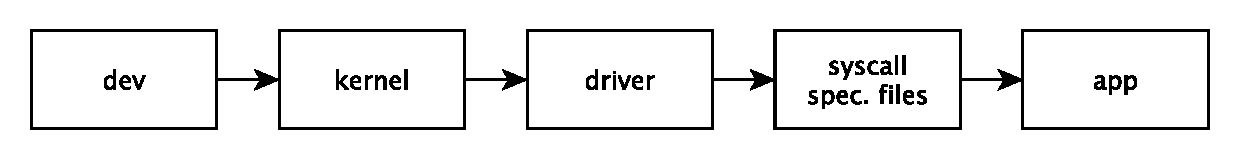
\includegraphics[width=1\linewidth]{./images/spec_files.pdf}
  \end{tabular}
\end{table}

\begin{quote}
\textit{Если процесс пользователя открывает для чтения обычный файл, то системные вызовы open и read обрабатываются встроенными в ядро функциями open и read соответственно. Если файл является специальным, то будут вызваны подпрограммы open и read, определенные в соответствующем драйвере устройства.}

\textit{После того, как по inode ФС распознает, что данный файл является специальным, ядро использует старший номер специального файла как индекс в конфигурационной таблице драйверов устройств. Элементом таблицы является структура, элементы которой содержат указатели на функции соответствующего драйвера. Младший номер передается драйверу, поддерживающему несколько устройств, как дополнительный параметр, указывающий конкретное устройство.}
\end{quote}

Имеется 2 типа файлов устройств:
\begin{enumerate}
	\item Символьные --- небуферизуемые (non-buffered).
	\item Блочные --- буферизуемые (устройства вторичной памяти).
\end{enumerate}

Связь имени специального файла с конкретным внешним устройством обеспечивает inode: есть поле dev\_t i\_rdev.

Тип специального файла задает поле mode. Для специального блок-ориентированного файла в этом поле устанавливается маска 06000, для байт-ориентированного 020000.

\begin{quote}

На структуры, описывающие устройства, ссылается inode:

\begin{lstlisting}
	struct inode {
    ...
    union {
        ...
        struct block_device    *i_bdev;
        struct cdev        *i_cdev;
        ...
    };
    ...
} __randomize_layout;
\end{lstlisting}

Таким образом, структуры block\_device (для блочных устройств) и cdev (для символьных устройств) определены в файловой системе Linux.

\begin{lstlisting}
	struct cdev {
    ...
    struct module *owner;
    const struct file_operations *ops;
    struct list_head list;
    dev_t dev;
    ...
} __randomize_layout;
\end{lstlisting}

Символьные устройства для регистрации в системе (нужных операций) используют структуру file\_operations. При создании символьного устройства в данной структуре нужно заполнить только два поля: ops и owner (обязательное значение - THIS\_MODULE).

\begin{lstlisting}
	struct block_device {
    dev_t            bd_dev; 
    ...
    struct inode *        bd_inode; 
    struct super_block *    bd_super;
    ...
    struct gendisk *    bd_disk; // (определяет устройство (специализированный интерфейс), ссылается на struct block_device_operations)
    ...
} __randomize_layout;
\end{lstlisting}

Чтобы сделать блочные устройства доступными для ядра, драйверы блочных устройств регистрируются в ядре с помощью функции register\_blkdev, но с версии 2.6.0 этот вызов необязателен и нужен только для динамического выделения старшего номера и создания записи в /proc/devices.

\end{quote}

\section{Адресация внешних устройств и их идентификация в системе, тип dev\_t}

Устройство --- специальный файл, не можем идентифицировать его как обычный файл. В ядре используется тип dev\_t (<linux/types.h>) для того, чтобы определять (содержать) номера устройств. С версии 2.6.0 dev\_t 32-разрядный. Представляет число, в котором 12 бит --- для старшего номера, 20 --- для младшего. POSIX.1 определяет существование типа, но не его формат.

\textbf{Пример:} жёсткий диск --- устройство. Дисковое адресное пространство поделено на разделы (используются для монтирования ФС). Диск будет иметь старший номер (major id) --- идентификатор класса устройства, а его разделы --- младший номер (minor id).  

Код пользователя не должен делать предположений о внутренней организации номера устройства, а должен просто использовать набор макросов <linux/kdev\_t.h>, используемых для получения старшего и младшего номеров устройства.

\begin{lstlisting}
	MAJOR(dev_t dev);
	MINOR(dev_t dev);
\end{lstlisting}

Для преобразования в dev\_t по старшему и младшему номерам используется макрос:

\begin{lstlisting}
	MKDEV(int major, int minor);
\end{lstlisting}

До версии 2.6.0 количество номеров было ограничено: до 255 младших и до 255 старших. Позже ограничения были сняты.

Файлы устройств одного типа имеют одинаковые номера и различаются по номеру, который добавляется в конец имени. 

\textbf{Пример:} все файлы сетевых плат имеют номера Ethernet: eth0, eth1...

Если внутри /dev вызвать ls -l, увидим два числа через запятую --- старший и младший номера устройств. Если выполнить cat /proc/devices --- увидим старшие номера устройств, известные ядру.

\section{Выделение/освобождение номеров устройств}

Одно из первых действий, которое должен сделать драйвер при установке, например, символьного устройства, --- получение 1 или более номеров устройств для работы с ними. 

Для выделения символьного устройства нужно вызвать функцию

\begin{lstlisting}
	int register_chrdev_region(dev_t first, unsigned int count, char* name);
\end{lstlisting}

first --- начальный номер диапазона устройств, которые мы хотим выделить (minor). К нему нет требований.

count --- количество запрашиваемых номеров устройств. Если count > запрашиваемого диапазона, то может перейти на следующий старший номер. Все будет работать до тех пор, пока запрашиваемый диапазон доступен. 

name --- имя номера устройства, связанного с диапазоном. Можно увидеть в /proc/devices и sysfs.

Возвращает 0, если успех, отрицательное число, если ошибка. 

Функция эффективна, если заранее известно конкретное устройство, которому нужен номер. Но часто неизвестно, какой старший номер использует конкретное устройство.

Есть тенденция по переходу на использование динамически разделяемых номеров устройств:

\begin{lstlisting}
	int alloc_chrdev_region(dev_t* dev, unsigned int first_minor, unsigned int count, char* name);
\end{lstlisting}

dev --- только выходной параметр, содержит первый номер в выделенном диапазоне при успехе. firstminor --- первый младший номер (нужен для идентификации устройства).

Для освобождения используется:

\begin{lstlisting}
	int unregister_chrdev_region(dev_t first, unsigned int count);
\end{lstlisting}

\section{Статическое выделение номеров устройств}
Некоторые старшие номера назначаются большинству обычных устройств статически (см. Documentation/devices.txt). 

\begin{table}[H]
\begin{center}
\begin{tabular}{|c|l|}
\hline
Старший номер & \multicolumn{1}{c|}{Тип устройства} \\ \hline
1             & Оперативная память                  \\ \hline
2             & Дисковод floppy                     \\ \hline
3             & 1-ый контроллер жёстких IDE-дисков  \\ \hline
4             & Терминалы                           \\ \hline
5             & Терминалы                           \\ \hline
6             & Принтеры (параллельный код)         \\ \hline
8             & Жёсткие SCSI-диски                  \\ \hline
13            & Мышь                                \\ \hline
14            & Звуковые карты                      \\ \hline
22            & 2-ой контроллер жёстких IDE-дисков  \\ \hline
\end{tabular}
\end{center}
\end{table}

\newpage

\section{Система прерываний: типы прерываний и их особенности}

Система прерываний включает в себя:
\begin{enumerate}
	\item Системные вызовы (синхронные --- возникают в процессе выполнения программы, вызываются соответствующей командой).
	\item Исключения (синхронные --- возникают в процессе выполнения программы, переполнение стека/деление на 0...).
	\item Аппаратные прерывания (асинхронные --- не зависят ни от каких действий в системе, выполняются на высоких уровнях приоритетов, их выполнение нельзя прервать, задача --- информирование процессов о событиях в системе, от системного таймера/клавиатуры...).
\end{enumerate}

\textbf{Про таблицы прерываний:}

\begin{quote}	
	В 16-разрядной ОС существует таблица векторов прерываний --- таблица, содержащая векторы прерывания (far-адреса обработчиков прерывания). Она начинается с нулевого адреса, занимает 1 Мб. Вектор прерывания - смещение в этой таблице.
	
	В 32-разрядной ОС cуществует IDT (Interrupt Descriptor Table), нужная для получения адресов обработчиков прерываний, содержащая 8-байтовые дескрипторы прерываний, хранящие информацию о смещении к обработчику прерывания в соответствующем сегменте.
	
	В 64-разрядной ОС существует IDT и список прерываний --- запутанная система.
	
	В современных системах часть перываний относится к APIC, а часть к подсистеме ОС MSI (Message Signal Interrupts).
\end{quote}

\newpage

\section{Прерывания в последовательности ввода-вывода --- обслуживание запроса процесса на ввод-вывод}

\begin{table}[h!]
  \centering
  \begin{tabular}{p{1\linewidth}}
    \centering
    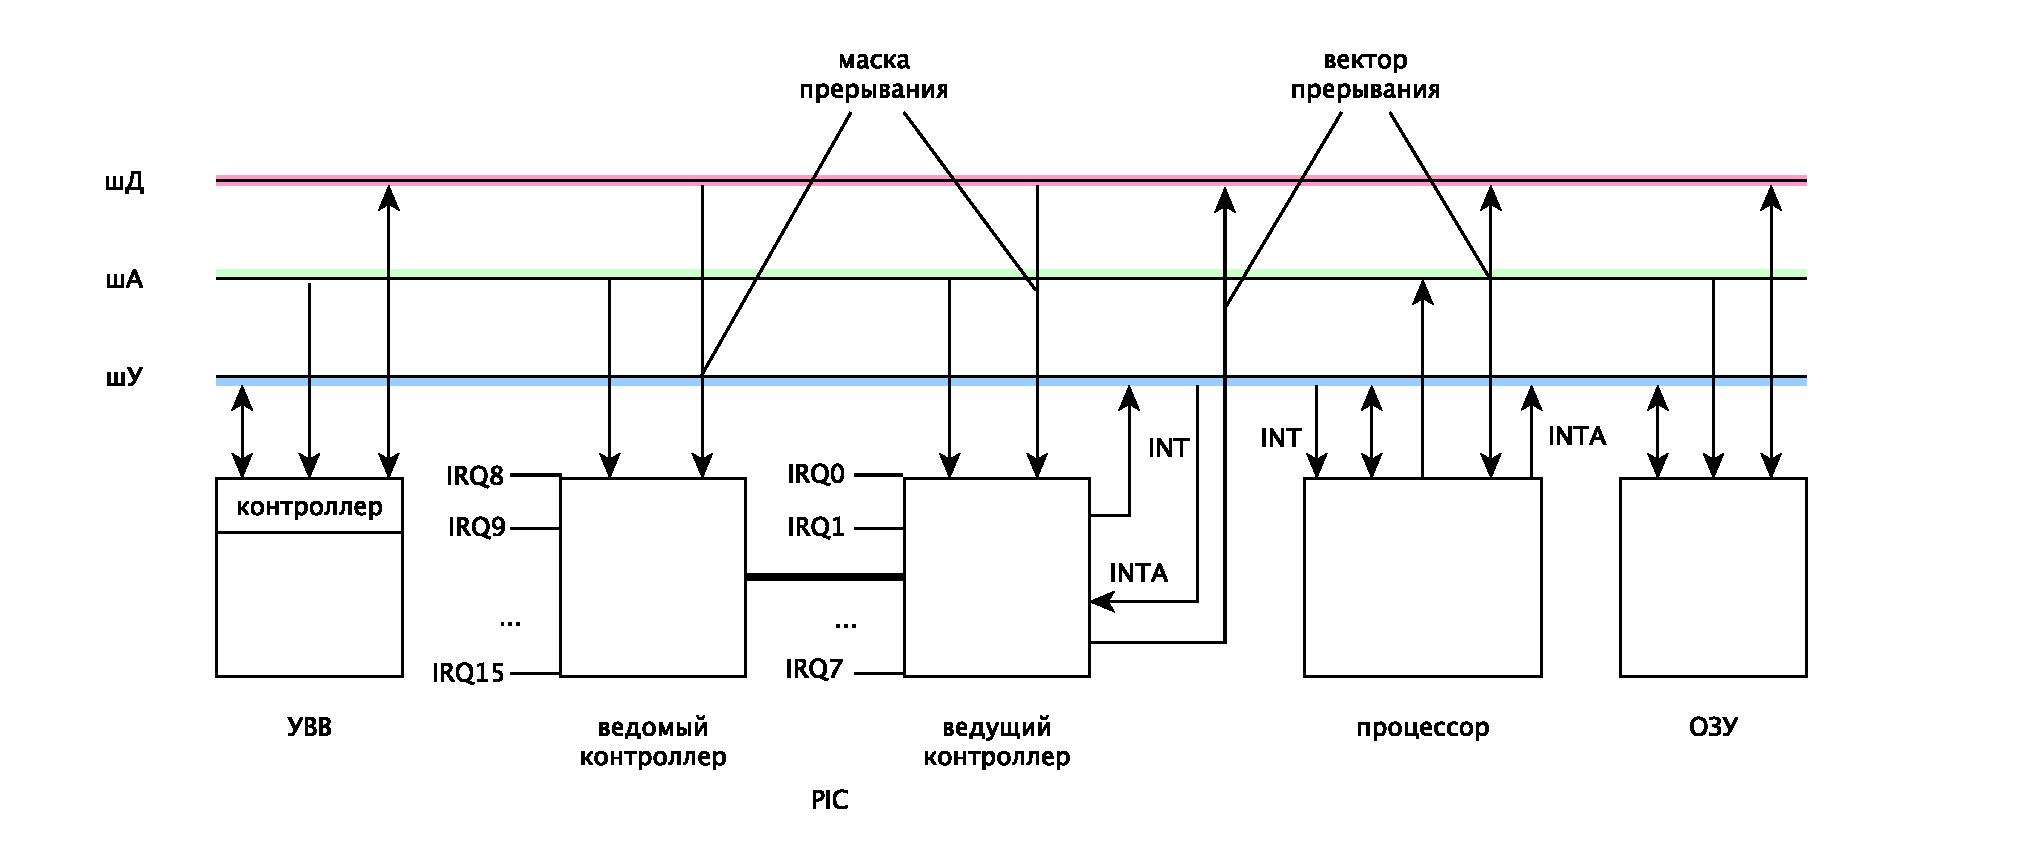
\includegraphics[width=0.9\linewidth]{./images/buses.pdf}
  \end{tabular}
\end{table}

Взаимодействие компьютера с внешними устройствами выполняется с помощью аппаратных прерываний --- идея распараллеливания действий, когда управление внешним устройством берёт на себя контроллер устройства (замена опроса готовности ВУ).

\begin{enumerate}
	\item Запрос приложения на ввод/вывод переводит систему в режим ядра.
	\item Подсистема ввода/вывода вызывает драйвер устройства (в драйвере есть 1 обработчик прерывания от данного устройства).
	\item По окончании операции ввода/вывода контроллер устройства формирует сигнал прерывания, приходящий на соответствующую линию прерывания контроллера прерываний.
	\item Контроллер формирует сигнал INT, который по ШУ идёт на выделенную ножку процессора.
	\item В конце цикла выполнения каждой команды (выборка-дешифрирование-выполнение) процессор проверяет наличие сигнала на ножке. Если есть сигнал, процессор выставляет на ШУ INTA.
	\item Контроллер отправляет по ШД вектор прерывания в регистры процессора.
	\item Процессор смещается относительно нулевого адреса и находит в таблице адрес обработчика.
\end{enumerate}

\begin{table}[h!]
  \centering
  \begin{tabular}{p{1\linewidth}}
    \centering
    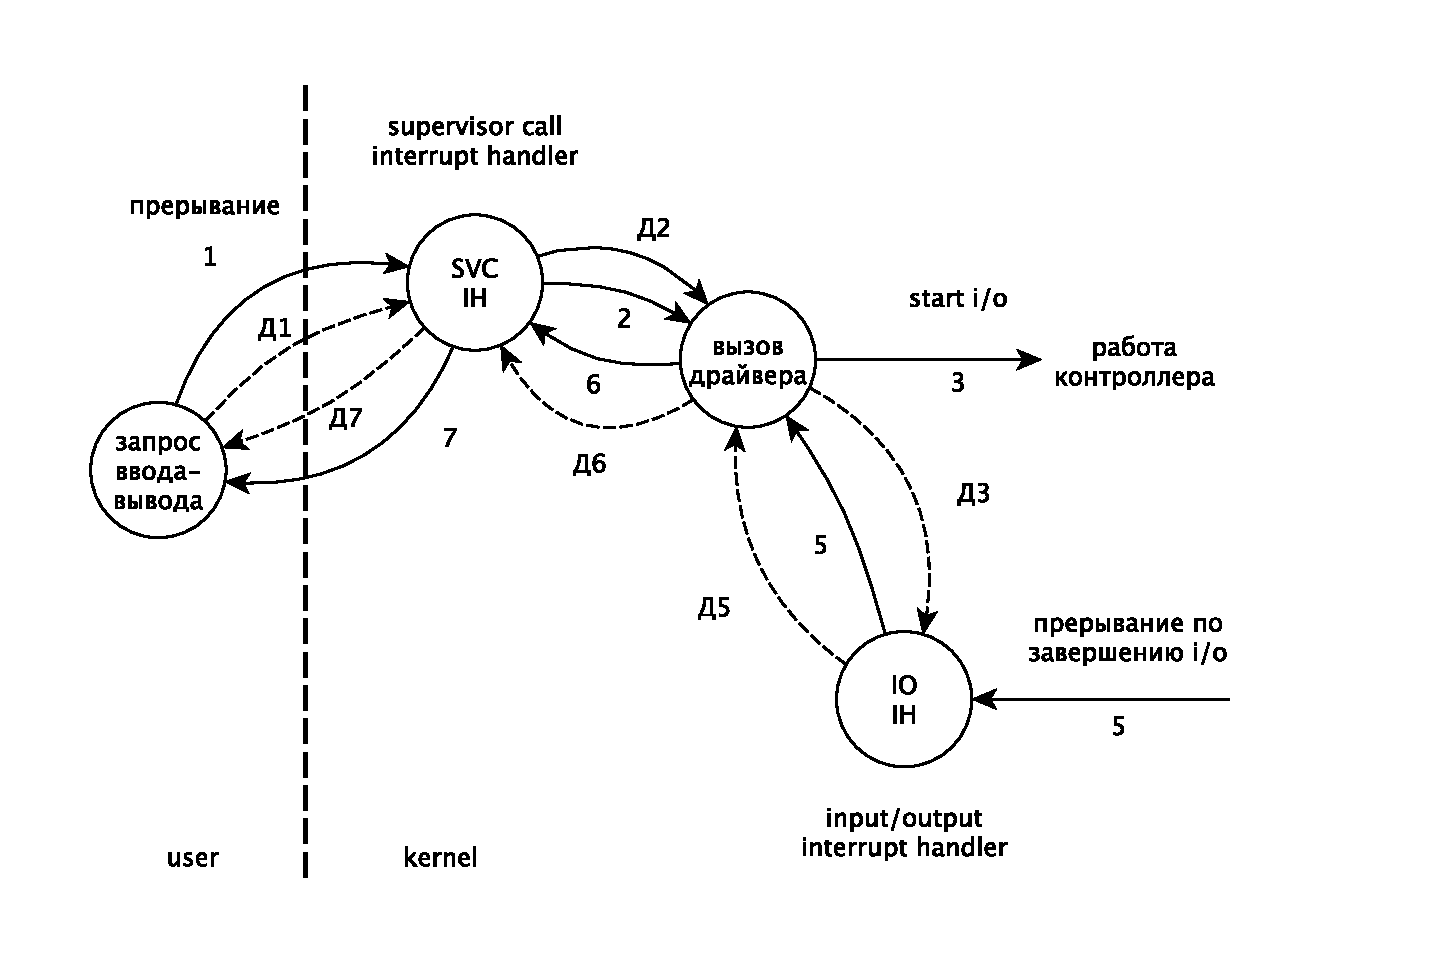
\includegraphics[width=0.8\linewidth]{./images/driver.pdf}
  \end{tabular}
\end{table}

\section{Быстрые и медленные прерывания}

Выделяются быстрые и медленные аппаратные прерывания. Быстрые --- выполняются атомарно, не делятся на части, в современных системах это только прерывание от системного таймера. Медленные --- все остальные, делятся на 2 части.

Любые АП выполняются на самом высоком уровне приоритета (самый высокий --- системный таймер, выше него только migration для перебалансировки нагрузки между процессорами и power при падении напряжения --- система отключается от питания и не может работать).

Аппаратные прерывания --- важнейшие в системе, поэтому, чтобы исключить в многопроцессорных системах ошибки обработки данных, поступающих от внешних устройств, на том ядре, на котором обрабатывается прерывание, запрещаются все остальные прерывания, а в системе запрещаются все прерывания по данной линии IRQ. Никакая другая работа на данном процессоре выполняться не может, что негативно сказывается на производительности и отзывчивости системы, поэтому АП не могут выполняться длительное время. Поэтому работа, которую выполняют обработчики прерываний, делится на 2 части.

Эти 2 части --- top\_half и bottom\_half. top\_half (interrupt handler) копирует данные устройства в специальный буфер, инициализирует отложенное действие bottom\_half (softirq, tasklet или workqueue) и завершается. top\_half должен выполниться быстро, так как при этом игнорируются остальные прерывания. bottom\_half выполняется при разрешённых остальных прерываниях и делает всю остальную обработку прерывания.

\section{Обработчики аппаратных прерываний: регистрация в системе --- функция и ее параметры, примеры}

Основная задача обработчика прерывания --- передача данных по шине данных устройства, если была запрошена операция чтения. Даже если была запрошена операция записи, устройство все равно оправляет по шине данных информацию об успешности операции. Чтобы обработать ее, обработчик должен сохранять информацию, поступающую от устройства в буфер ядра. Затем эта информация поступит приложению, запросившему ввод/вывод.

Системная функция для регистрации обработчика прерывания:

\begin{lstlisting}
	typedef irqreturn_t (*irq_handler_t)(int, void *); 
	
	int request_irq(unsigned int irq, irq_handler_t handler, unsigned long flags, const char* name, void *dev);
\end{lstlisting}

irq --- номер линии прерывания. handler --- обработчик прерывания. flags --- флаги. name --- имя устройства/обработчика. dev - указатель на некоторый объект, используется для освобождения линии прерывания от указанного обработчика:

\begin{lstlisting}
	const void *free_irq(unsigned int irq, void *dev_id);
\end{lstlisting}

\textbf{Пример:}
\begin{lstlisting}
	rc = request_irq(IRQ_NUMBER, interrupt_handler, IRQF_SHARED, "tasklet_interrupt_handler", interrupt_handler);
\end{lstlisting}

Флаг IRQF\_SHARED указывает, что данная линия прерывания может быть разделена несколькими обработчиками. IRQF\_TIMER --- флаг, маскирующий данное прерывание как прерывание от таймера. IRQF\_PROBE\_SHARED --- устанавливается абонентами, если возможны проблемы при совместном использовании линии.

\section{Тасклеты --- объявление, планирование}

Тасклет --- специальный тип softirq. Тасклеты представлены двумя типами отложенных прерываний: HI\_SOFTIRQ  и TASKLET\_SOFTIRQ.

\textbf{Тасклет не может выполняться параллельно, выполняется атомарно на том же процессоре, на котором выполняется обработчик вызвавшего его прерывания. Инициализируется как статически, так и динамически. Выполняется в контексте прерывания --- нельзя использовать средства взаимоисключения, кроме spinlocks. Выполняется ksofirqd. Является упрощённым интерфейсом softirq.}

Определена структура:

\begin{lstlisting}
struct tasklet_struct
{
	struct tasklet_struct *next;
	unsigned long state;
	atomic_t count;
	bool use_callback;
	union {
		void (*func)(unsigned long data);
		void (*callback)(struct tasklet_struct *t);
	};
	unsigned long data;
};
\end{lstlisting}

Тасклеты в отличие от softirq могут быть зарегистрированы как статически, так и динамически. Статически тасклеты создаются с помощью двух макросов (man 6.2.1):

\begin{lstlisting}
#define DECLARE_TASKLET(name, _callback)		\
struct tasklet_struct name = {				\
	.count = ATOMIC_INIT(0),			\
	.callback = _callback,				\
	.use_callback = true,				\
}
#define DECLARE_TASKLET_DISABLED(name, _callback)	\
struct tasklet_struct name = {				\
	.count = ATOMIC_INIT(1),			\
	.callback = _callback,				\
	.use_callback = true,				\
}
\end{lstlisting}

Оба  макроса статически создают экземпляр структуры struct tasklet\_struct с указанным именем (name). Например,

\begin{lstlisting}
DECLARE_TASKLET(my_tasklet, tasklet_handler);
\end{lstlisting}

Эта строка эквивалентна следующему объявлению:
\begin{lstlisting}
struct tasklet_struct rny_tasklet = {NULL, 0, ATOMIC_INIT(0), tasklet_handler};
\end{lstlisting}

В данном примере создается тасклет с именем my\_tasklet, который разрешен для выполнения. Функция tasklet\_handler будет обработчиком этого тасклета. Поле dev отсутствует в текущих ядрах.

При динамическом создании тасклета объявляется указатель на
struct tasklet\_struct, а затем для инициализации вызывается функция:
\begin{lstlisting}
extern void tasklet_init(struct tasklet_struct *t, void (*func)(unsigned long), unsigned long data);
\end{lstlisting}

Пример:
\begin{lstlisting}
tasklet_init(t, tasklet_handler, data);
\end{lstlisting}   

Тасклеты должны быть зарегестрированы для выполнения. Тасклеты могут быть запланированы на выполнение функциями:
\begin{lstlisting}
tasklet_schedule(struct tasklet_struct *t); 
tasklet_hi_sheduler(struct tasklet_struct *t);
\end{lstlisting}  

Когда тасклет запланирован, ему выставляется состояние TASKLET\_STATE\_SCHED, и тон добавляется в очередь. Пока он находится в этом состоянии, запланировать его еще раз не получится, т.е. в этом случае просто ничего не произойдет. Тасклет не может находиться сразу в нескольких местах очереди на планирование, которая организуется через поле next структуры tasklet\_struct. После того, как тасклет был запланирован, он выполниться только один раз.

Свойства:
\begin{enumerate}
	\item Если вызывается функция tasklet\_schedule(), то после этого тасклет гарантированно будет выполнен на каком-либо процессоре хотя бы один раз. 
	\item Если тасклет уже запланирован, но его выполнение все еще не запущено, он будет выполнен только один раз. 
	\item Если этот тасклет уже запущен на другом процессоре (или schedule вызывается из самого тасклета), выполнение переносится на более поздний срок. 
	\item Тасклет строго сериализован по отношению к самому себе, но не по отношению к другим тасклетам. Если разработчик считает, что в данном тасклете нужно выполнить действия, которые могут выполняться в других таскоетах, он реализует взаимоисключение с помощью spinlocks.
\end{enumerate}

\begin{table}[]
\begin{center}
\begin{tabular}{|c|l|l|l|}
\hline
Критерии                                                            & \multicolumn{1}{c|}{softirq}                                                               & \multicolumn{1}{c|}{tasklet}                                                                    & \multicolumn{1}{c|}{workqueue}                                                           \\ \hline
Определение                                                         & \begin{tabular}[c]{@{}l@{}}10 шт. определено\\ в ядре статически\end{tabular}              & С + Д                                                                                           & С + Д                                                                                    \\ \hline
Сериализация                                                        & Да                                                                                         & Нет                                                                                             & Да                                                                                       \\ \hline
\begin{tabular}[c]{@{}c@{}}Возможность \\ паралл. вып.\end{tabular} & Да                                                                                         & Нет                                                                                             & Да                                                                                       \\ \hline
Выполнение                                                          & \begin{tabular}[c]{@{}l@{}}В контексте спец.\\ потоков ядра (ksoftirqd)\end{tabular} & \begin{tabular}[c]{@{}l@{}}В контексте\\ запланировавшего\\ обраб. прерыв.\end{tabular} & \begin{tabular}[c]{@{}l@{}}В контексте спец.\\ потоков ядра (kworker)\end{tabular} \\ \hline
Блокируются                                                         & ???                                                                                        & Нет                                                                                             & Да                                                                                       \\ \hline
\end{tabular}
\end{center}
\end{table}

\section{spin\_lock}

Race condition --- условия гонок: процессы выполняются с разной скоростью и пытаются получить доступ к разделяемым переменным. 

Аппаратная реализация взаимоисключения --- test\_and\_set. Атомарная функция, реализующая как неделимое действие проверку и установку значения в памяти. По сути, читает значение переменной b, копирует его в a, устанавливает b значение true. Считается, что это не приведет к бесконечному откладыванию. 

Использование test\_and\_set в цикле проверки значения переменной называется циклической блокировкой. Spin-блокировки --- активное ожидание на процессоре (время непроизводительно расходуется на проверку флага другого процессора). Реализация test\_and\_set связана с блокировкой локальной шины памяти, в результате один поток может занять шину на длительное время, что понижает отзывчивость (решение --- 2 вложенных цикла, если переменная занята --- выполняется обычный цикл без блокировки шины).

\begin{lstlisting}
	void spin_lock(spin_lock_t* c)
	{
		while (test_and_set(*c) != 0)
		{
			/* ресурс занят */
			
			/*
			while (*c != 0) 
			{
			...
			}
			*/
		}
	}
	
	void spin_unlock(spin_lock_t* c)
	{
		*c = 0;
	}
\end{lstlisting}

Циклическую блокировку может удерживать только 1 поток. Захваченная --- в состоянии contended. Если другой поток пытается захватить уже захваченную, то блокировка находится в состоянии конфликта, а поток выполняет цикл проверки busy\_loop. Блокировка должна быть связана с тем, что она блокирует. Запрещаются данные (разделяемый ресурс), а не код.

\textbf{Пример из лабораторной:}

\begin{lstlisting}
#include <linux/kernel.h>
#include <linux/module.h>
#include <linux/interrupt.h>
#include <linux/slab.h>
#include <asm/io.h>

#include "ascii.h"

#define IRQ_NUMBER 1

MODULE_LICENSE("GPL");
MODULE_AUTHOR("Karpova Ekaterina");

struct tasklet_struct *tasklet;
char tasklet_data[] = "key pressed";

void tasklet_func(unsigned long data)
{
    printk(KERN_INFO "+: -----------------------");
    printk(KERN_INFO "+: tasklet began");
    printk(KERN_INFO "+: tasklet count = %u", tasklet->count.counter);
    printk(KERN_INFO "+: tasklet state = %lu", tasklet->state);

    printk(KERN_INFO "+: key code - %d", data);
    if (data < ASCII_LEN)
        printk(KERN_INFO "+: key press - %s", ascii[data]);
    if (data > 128 && data < 128 + ASCII_LEN)
        printk(KERN_INFO "+: key release - %s", ascii[data - 128]);
        
    printk(KERN_INFO "+: tasklet ended");
    printk(KERN_INFO "+: -----------------------");
}

static irqreturn_t my_irq_handler(int irq, void *dev_id)
{
  int code;
  printk(KERN_INFO "+: my_irq_handler called\n");
  
  if (irq != IRQ_NUMBER)
  {
    printk(KERN_INFO "+: irq not handled");
    return IRQ_NONE;
  }
  
  printk(KERN_INFO "+: tasklet state (before schedule) = %lu",
                 tasklet->state);
  code = inb(0x60);
  tasklet->data = code;
  tasklet_schedule(tasklet);
  printk(KERN_INFO "+: tasklet scheduled");
  printk(KERN_INFO "+: tasklet state (after schedule) = %lu",
                  tasklet->state);
                  
  return IRQ_HANDLED;
}

static int __init my_init(void) 
{
  if (request_irq(IRQ_NUMBER, my_irq_handler, IRQF_SHARED, "tasklet_irq_handler", (void *) my_irq_handler))
  {
    printk(KERN_ERR "+: cannot register irq handler\n");
    return -1;
  }
  
  tasklet = kmalloc(sizeof(struct tasklet_struct), GFP_KERNEL);

  if (tasklet == NULL)
  {
        printk(KERN_ERR "+: kmalloc error");
        return -1;
  }

  tasklet_init(tasklet, tasklet_func, (unsigned long)tasklet_data);
  
  printk(KERN_INFO "+: module loaded\n");
  return 0;
}

static void __exit my_exit(void)
{
  tasklet_kill(tasklet);
  free_irq(IRQ_NUMBER, my_irq_handler);

  printk(KERN_INFO "+: module unloaded\n");
}

module_init(my_init);
module_exit(my_exit);

\end{lstlisting}






